\documentclass[UTF8]{ctexart}
\usepackage{graphicx}
\usepackage{listings}

\title{实验七报告}
\author{唐灵\\519030910052\\F1903002}
\date{\today}
\begin{document}
    \maketitle
    \begin{abstract}
        这是电工导C课程的第六次实验
    \end{abstract}
    \section{实验概览}
        本次实验是一次整合,整合前半期到内容,实现建立图片以及网页的索引,并通过flask网页框架进行实现。最后一步是添加css样式,让我们的结果更加的好看(虽然最后实际上是变得更丑了)

        由于对于其他部分的实现,在以前的报告已经讲的非常清楚了,本次报告主要着重于对于网页部分的实现的表述。
    \section{实验环境}

        \begin{figure}[ht]
            \centering
            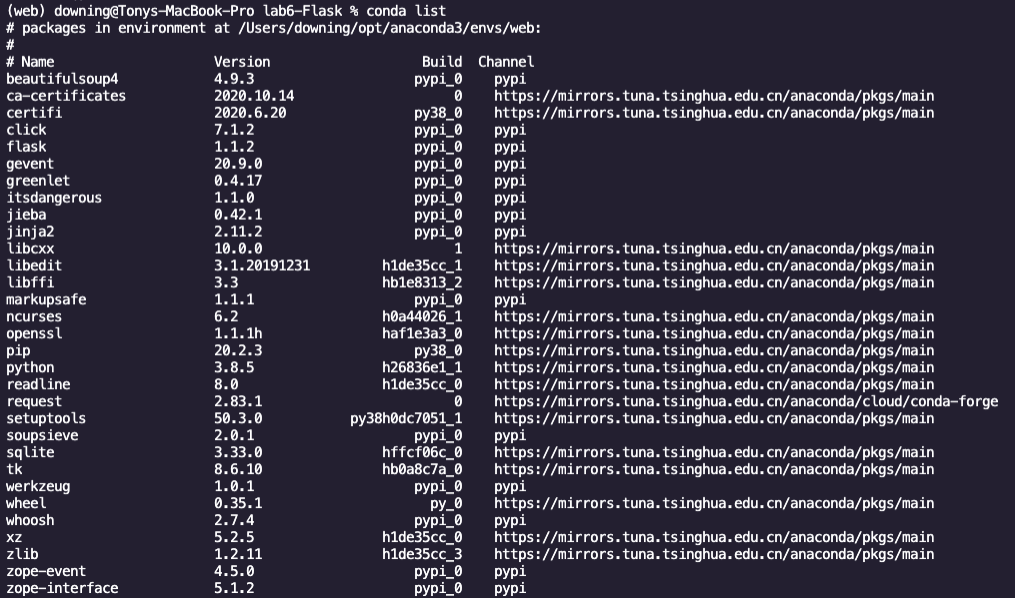
\includegraphics[scale=0.15]{img/env.png}
            \caption{实验运行环境}
        \end{figure} 
        本次作业文本检索部分使用了whoosh,具体原因已经在实验六中进行过说明,具体原因不再重复。
        
        其他部分和课程要求内容完全一致,在本地环境中使用anaconda3完成实验,
        python的版本为3.8.5,具体环境环境如上图。     

    \section{练习解决思路}
        \subsection{总体思路}
            总体的实现思路大致可以描述如下:
            \begin{enumerate}
                \item 服务器初始化根目录为搜索页面,通过 search.html 渲染模版。
                \item 程序猿从浏览器发起搜索,通过搜索页面向服务器发送请求,通过重定向到结果页面(由于页面设置,结果页面本身也是搜索页面),
                请求中后缀有"keyword"参数。
                \item 服务器通过获得keyword参数,再将keyword传入到search()函数,并返回搜索结果,这个函数来自于搜索模块,这个模块会对之前创建的索引进行搜索
                ,并返回所有的搜索结果,这个结果足够覆盖结果页面中我们用到的所有信息,并且已经进行过高亮处理。
                \item 将返回的搜索结果作为参数传入进网页模版 result.html 进行渲染,得到我们的搜索结果,再传回给浏览器。
            \end{enumerate}

            对于图片和网页的索引,在这个层面来讲没有任何不同,所以在上述过程中省略掉在源文件中出现的doc和img后缀。

        \subsection{网页框架实现思路}
            具体思路基本上按照以上的逻辑构建,截图如下:

            \begin{figure}[ht]
                \centering
                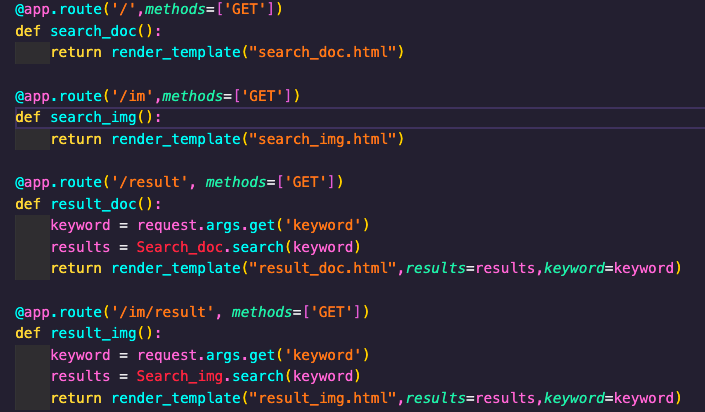
\includegraphics[scale=0.15]{img/app.png}
                \caption{网页逻辑}
            \end{figure}
        \subsection{网页模版实现思路}
            网页模版要接受搜索结果传来的列表类型参数,然后进行循环打印输出,相较于上一次的不同,本次使用了css使我们的页面更加的好看,

            由于网页结构还是较为简单,选择选用内嵌,与讲css样式写进head的两种方式来得到我们希望的效果,对于图片,使用max-width等方式来使得页面显示能够随比例的变化而变化。
            \begin{figure}[ht]
                \centering
                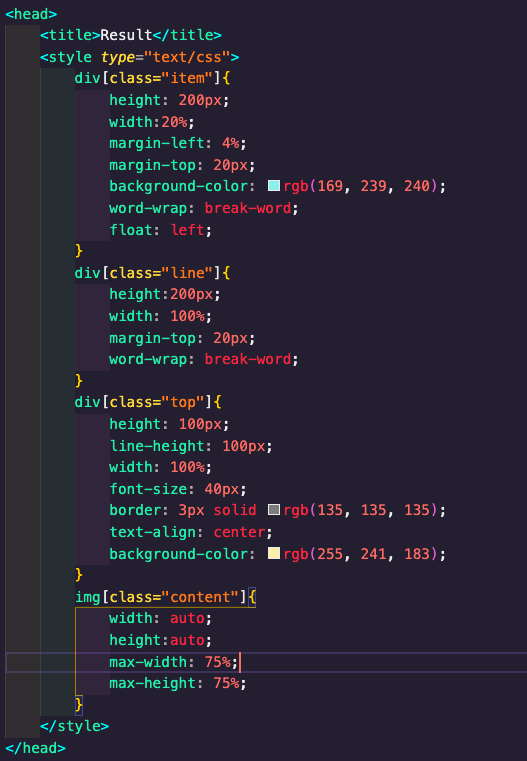
\includegraphics[scale=0.4]{img/css.png}
                \caption{css样式设计}
            \end{figure}
    \section{代码运行结果}
        最后显示一些搜索结果。

        \begin{figure}[ht]
            \centering
            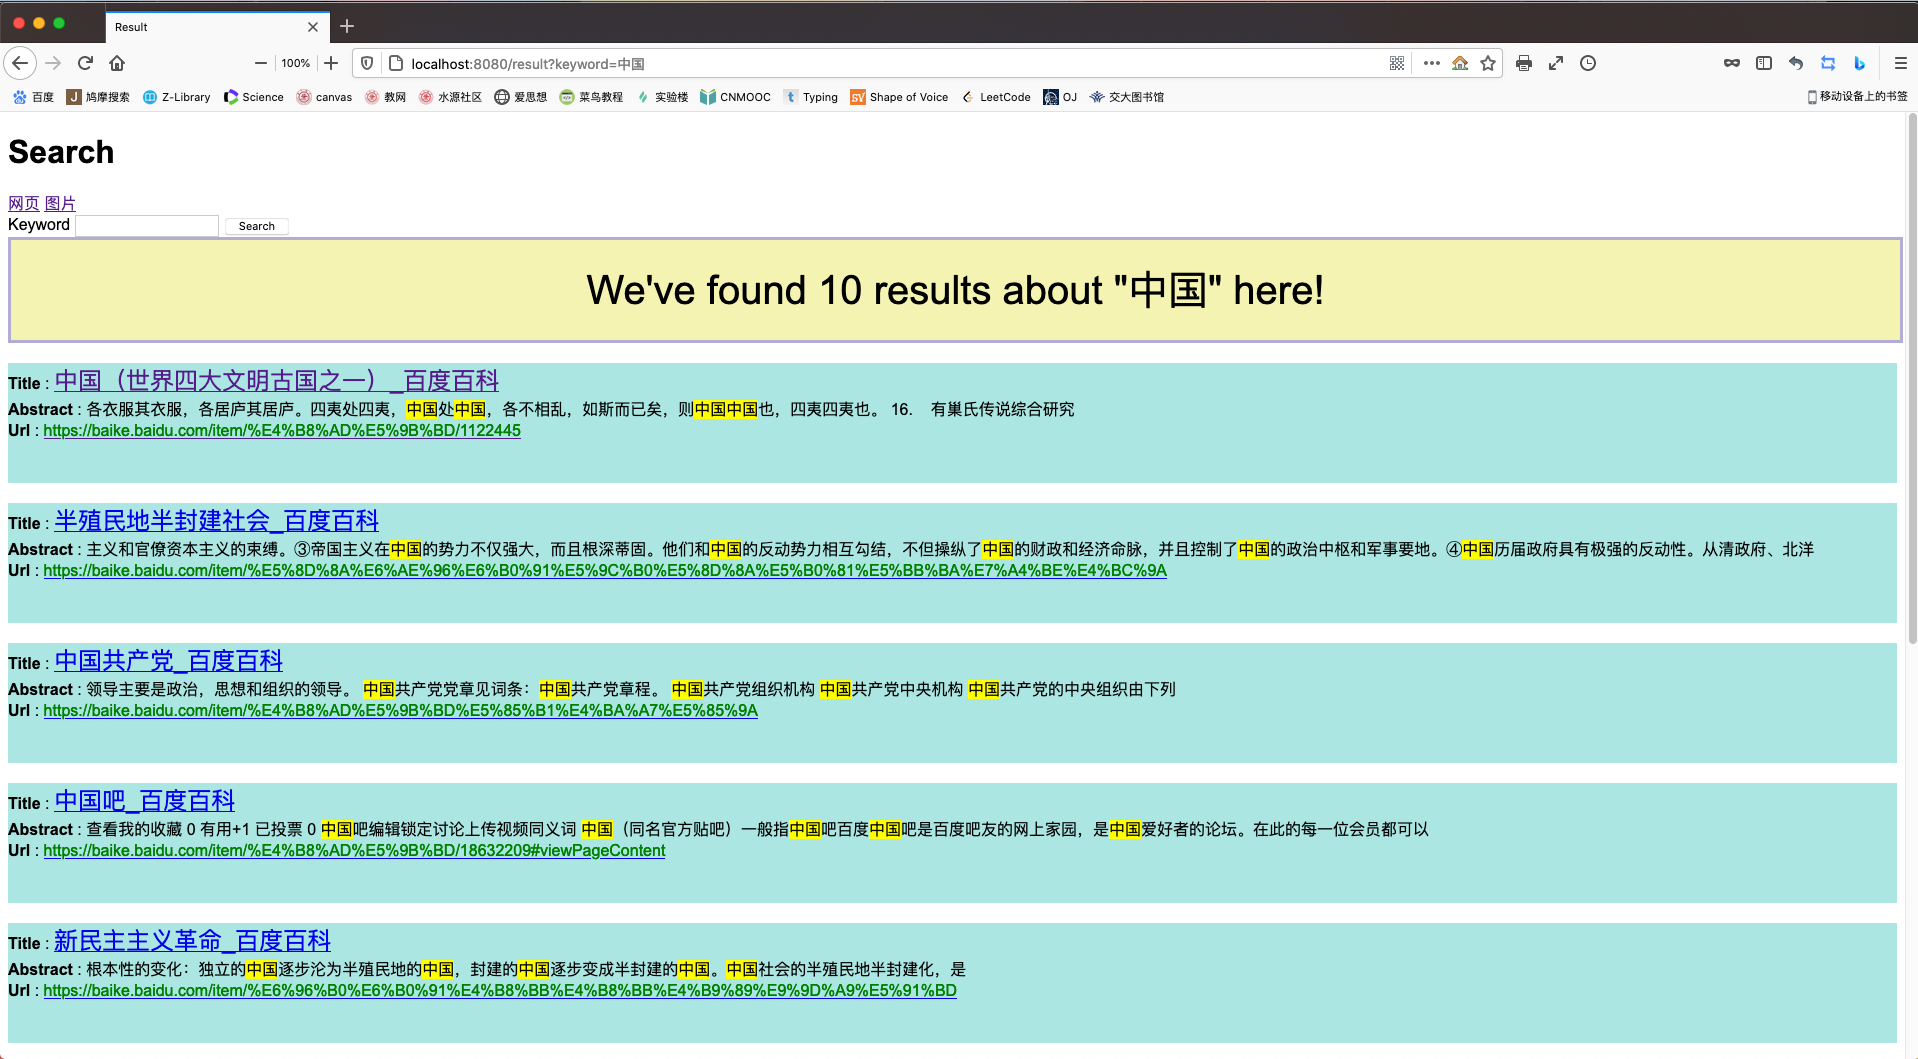
\includegraphics[scale=0.14]{img/doc.png}
            \caption{网页文档搜索结果}
        \end{figure}

        \begin{figure}[ht]
            \centering
            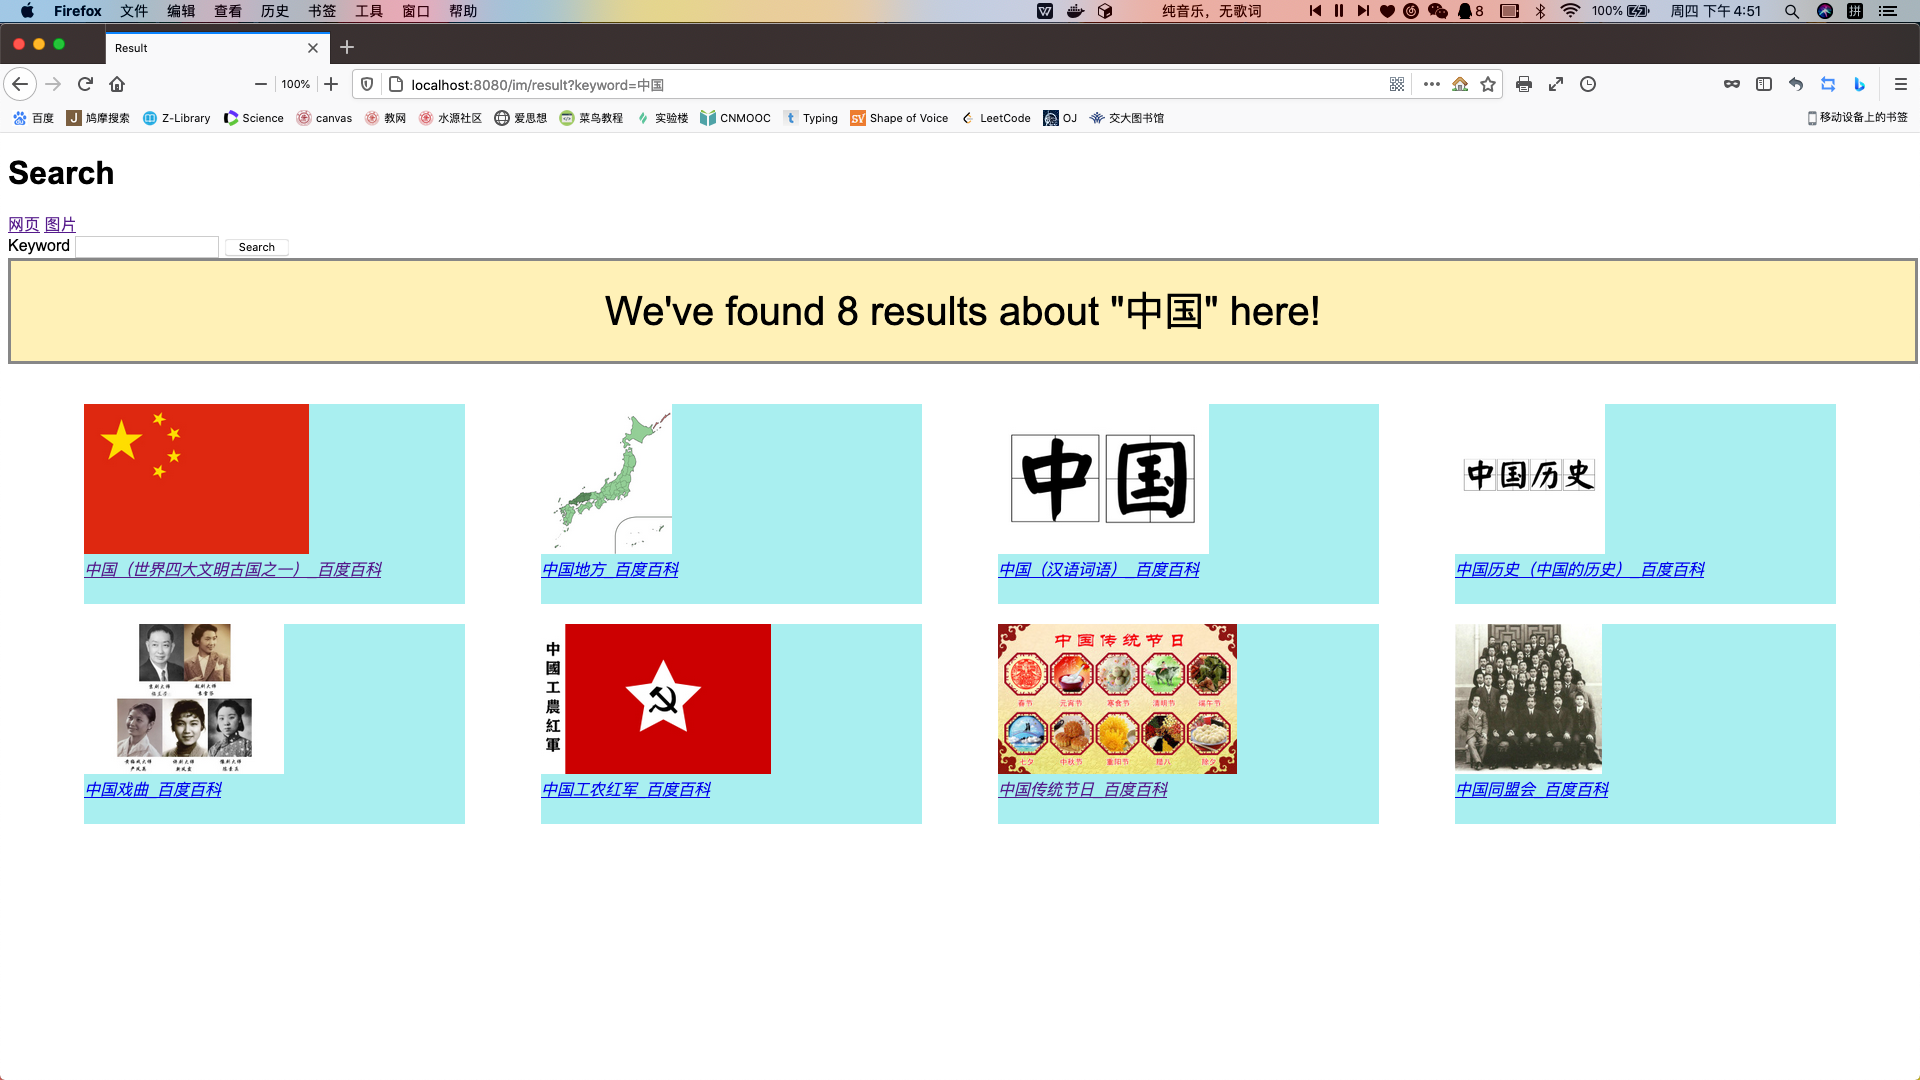
\includegraphics[scale=0.14]{img/img.png}
            \caption{图片搜索结果}
        \end{figure}


\end{document}